\documentclass[border=8pt]{standalone}
\usepackage{amsmath}
\usepackage{amssymb}
\usepackage{tikz}
\usetikzlibrary{arrows.meta,calc,decorations.pathreplacing,decorations.pathmorphing,patterns,shapes.geometric,positioning,shadings}

\begin{document}
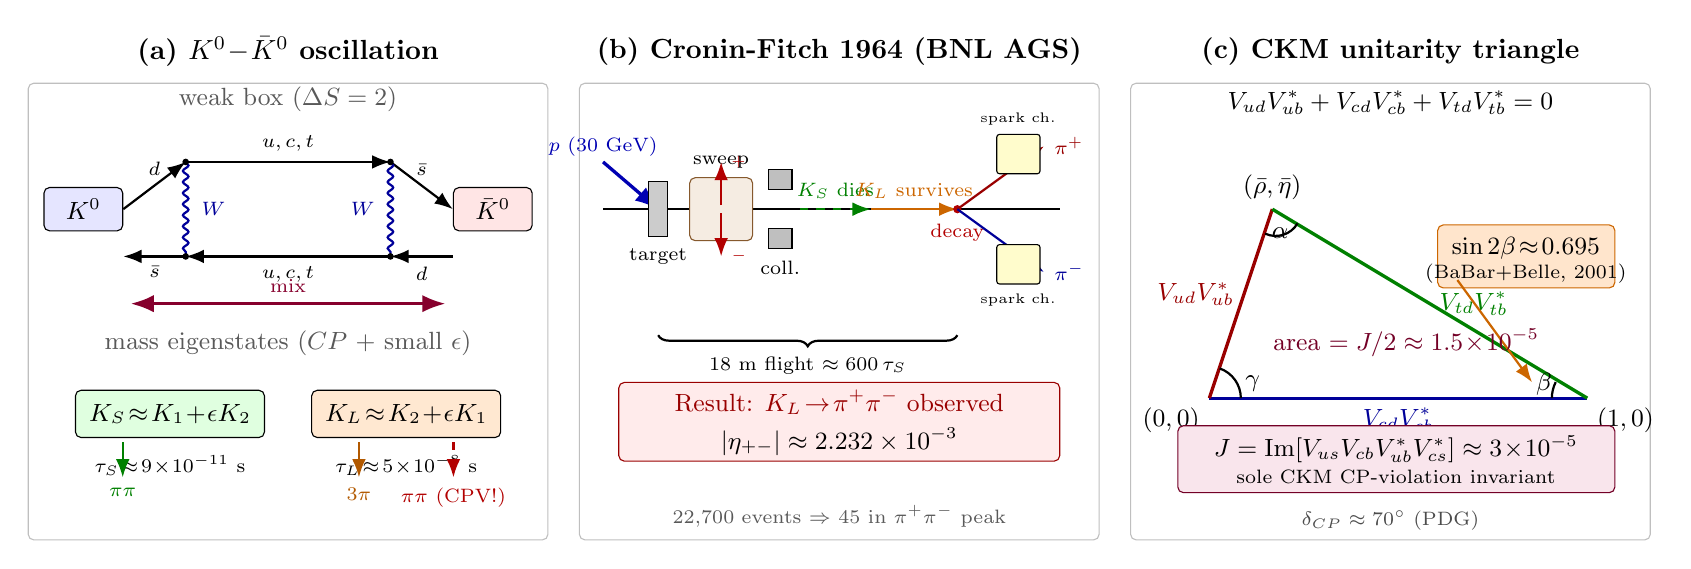
\begin{tikzpicture}[>=Latex]

% =============================================================
% PANEL 1 (LEFT): K0 - Kbar0 oscillation via box diagram
% =============================================================
\begin{scope}[xshift=0cm,yshift=0cm]
  % Panel title
  \node[font=\bfseries] at (3.0,5.6) {(a) $K^0\!-\!\bar K^0$ oscillation};

  % Frame
  \draw[gray!50,rounded corners=2pt] (-0.3,-0.6) rectangle (6.3,5.2);

  % --- Top: box diagram ---
  \node[font=\small,gray!70!black] at (3.0,5.0) {weak box ($\Delta S=2$)};

  % Outer K0 on left, Kbar0 on right
  \node[draw,rounded corners=2pt,fill=blue!10,minimum width=1.0cm,minimum height=0.55cm,font=\small] (K0) at (0.4,3.6) {$K^0$};
  \node[draw,rounded corners=2pt,fill=red!10,minimum width=1.0cm,minimum height=0.55cm,font=\small] (Kb0) at (5.6,3.6) {$\bar K^0$};

  % Box vertices
  \coordinate (v1) at (1.7,4.2);
  \coordinate (v2) at (4.3,4.2);
  \coordinate (v3) at (1.7,3.0);
  \coordinate (v4) at (4.3,3.0);

  % Quark lines (top: d, bottom: sbar)  --- internal up-type quarks u,c,t
  \draw[->,thick] (K0.east) -- node[above,font=\scriptsize]{$d$} (v1);
  \draw[->,thick] (v2) -- node[above,font=\scriptsize]{$\bar s$} (Kb0.west);
  \draw[<-,thick] (K0.east) ++ (0,-0.6) -- node[below,font=\scriptsize]{$\bar s$} ($(v3)+(0,0)$);
  \draw[<-,thick] ($(v4)+(0,0)$) -- node[below,font=\scriptsize]{$d$} ($(Kb0.west)+(0,-0.6)$);

  % Internal quark lines (top: u/c/t connection)
  \draw[->,thick] (v1) -- node[above,font=\scriptsize]{$u,c,t$} (v2);
  \draw[<-,thick] (v3) -- node[below,font=\scriptsize]{$u,c,t$} (v4);

  % W boson exchanges (vertical, wavy)
  \draw[decorate,decoration={snake,amplitude=1pt,segment length=4pt},thick,blue!60!black]
    (v1) -- node[right=2pt,font=\scriptsize]{$W$} (v3);
  \draw[decorate,decoration={snake,amplitude=1pt,segment length=4pt},thick,blue!60!black]
    (v2) -- node[left=2pt,font=\scriptsize]{$W$} (v4);

  % Vertices
  \foreach \p in {v1,v2,v3,v4} \fill (\p) circle (1.2pt);

  % Double-arrow indicating mixing
  \draw[<->,very thick,purple!70!black] (1.0,2.4) -- node[above,font=\scriptsize]{mix} (5.0,2.4);

  % --- Lower: mass eigenstates ---
  \node[font=\small,gray!70!black] at (3.0,1.9) {mass eigenstates ($CP$ + small $\epsilon$)};

  \node[draw,rounded corners=2pt,fill=green!12,minimum width=2.4cm,minimum height=0.6cm,font=\small] (KS) at (1.5,1.0) {$K_S \!\approx\! K_1\!+\!\epsilon K_2$};
  \node[draw,rounded corners=2pt,fill=orange!18,minimum width=2.4cm,minimum height=0.6cm,font=\small] (KL) at (4.5,1.0) {$K_L \!\approx\! K_2\!+\!\epsilon K_1$};

  % Lifetimes
  \node[font=\scriptsize] at (1.5,0.35) {$\tau_S\!\approx\!9\!\times\!10^{-11}$ s};
  \node[font=\scriptsize] at (4.5,0.35) {$\tau_L\!\approx\!5\!\times\!10^{-8}$ s};

  % Decays arrows
  \draw[->,thick,green!50!black] (KS.south) ++ (-0.6,-0.05) -- ++(0,-0.45) node[below,font=\scriptsize]{$\pi\pi$};
  \draw[->,thick,orange!70!black] (KL.south) ++ (-0.6,-0.05) -- ++(0,-0.45) node[below,font=\scriptsize]{$3\pi$};
  \draw[->,thick,red!70!black,dashed] (KL.south) ++ (0.6,-0.05) -- ++(0,-0.45) node[below,font=\scriptsize]{$\pi\pi$ (CPV!)};
\end{scope}

% =============================================================
% PANEL 2 (MIDDLE): Cronin-Fitch experiment schematic
% =============================================================
\begin{scope}[xshift=7cm,yshift=0cm]
  \node[font=\bfseries] at (3.0,5.6) {(b) Cronin-Fitch 1964 (BNL AGS)};
  \draw[gray!50,rounded corners=2pt] (-0.3,-0.6) rectangle (6.3,5.2);

  % Beam pipe baseline
  \draw[thick] (0.0,3.6) -- (5.8,3.6);

  % Proton beam from left
  \draw[->,very thick,blue!70!black] (-0.0,4.2) -- (0.7,3.6);
  \node[blue!70!black,font=\scriptsize] at (0.0,4.4) {$p$ (30 GeV)};

  % Target
  \node[draw,fill=gray!40,minimum width=0.18cm,minimum height=0.7cm,font=\tiny] (T) at (0.7,3.6) {};
  \node[font=\scriptsize] at (0.7,3.0) {target};

  % Sweeping magnet (charged particles deflected away)
  \draw[draw=brown!70!black,fill=brown!15,rounded corners=2pt] (1.1,3.2) rectangle (1.9,4.0);
  \node[font=\scriptsize] at (1.5,4.2) {sweep};
  \draw[->,thick,red!70!black] (1.5,3.6) ++(0.0,0.05) -- ++(0.0,0.55) node[right,font=\tiny]{$+$};
  \draw[->,thick,red!70!black] (1.5,3.6) ++(0.0,-0.05) -- ++(0.0,-0.55) node[right,font=\tiny]{$-$};

  % Collimator
  \draw[fill=gray!50] (2.1,3.85) rectangle (2.4,4.1);
  \draw[fill=gray!50] (2.1,3.10) rectangle (2.4,3.35);
  \node[font=\scriptsize] at (2.25,2.85) {coll.};

  % Neutral beam: KS dies, KL survives
  \draw[->,thick,green!50!black,dashed] (2.5,3.6) -- node[above,font=\scriptsize]{$K_S$ dies} (3.4,3.6);
  \draw[->,thick,orange!80!black] (3.4,3.6) -- node[above,font=\scriptsize]{$K_L$ survives} (4.5,3.6);

  % Decay vertex
  \fill[red!70!black] (4.5,3.6) circle (1.5pt);
  \node[font=\scriptsize,red!70!black] at (4.5,3.30) {decay};

  % Two pion tracks into spectrometer arms
  \draw[->,thick,red!60!black] (4.5,3.6) -- (5.6,4.4) node[right,font=\scriptsize]{$\pi^+$};
  \draw[->,thick,blue!60!black] (4.5,3.6) -- (5.6,2.8) node[right,font=\scriptsize]{$\pi^-$};

  % Spark chamber arms
  \draw[draw=black,fill=yellow!20,rounded corners=1pt] (5.0,4.05) rectangle (5.55,4.55);
  \draw[draw=black,fill=yellow!20,rounded corners=1pt] (5.0,2.65) rectangle (5.55,3.15);
  \node[font=\tiny] at (5.27,4.75) {spark ch.};
  \node[font=\tiny] at (5.27,2.45) {spark ch.};

  % Distance brace
  \draw[decorate,decoration={brace,amplitude=4pt,mirror},thick] (0.7,2.0) -- node[below=4pt,font=\scriptsize]{18 m flight $\approx 600\,\tau_S$} (4.5,2.0);

  % Result box
  \draw[draw=red!60!black,fill=red!8,rounded corners=2pt] (0.2,0.4) rectangle (5.8,1.4);
  \node[font=\small,red!60!black] at (3.0,1.15) {Result: $K_L\!\to\!\pi^+\pi^-$ observed};
  \node[font=\small] at (3.0,0.65) {$|\eta_{+-}|\approx 2.232\times 10^{-3}$};

  % Title underline accent
  \node[font=\scriptsize,gray!70!black] at (3.0,-0.3) {$22{,}700$ events $\Rightarrow$ 45 in $\pi^+\pi^-$ peak};
\end{scope}

% =============================================================
% PANEL 3 (RIGHT): CKM unitarity triangle
% =============================================================
\begin{scope}[xshift=14cm,yshift=0cm]
  \node[font=\bfseries] at (3.0,5.6) {(c) CKM unitarity triangle};
  \draw[gray!50,rounded corners=2pt] (-0.3,-0.6) rectangle (6.3,5.2);

  % Closure equation
  \node[font=\small] at (3.0,4.95) {$V_{ud}V_{ub}^*+V_{cd}V_{cb}^*+V_{td}V_{tb}^*=0$};

  % Vertices of normalized triangle (rho-eta plane)
  % A = (0,0)  C = (1,0)  B = (rho, eta) ~ (0.16, 0.35)
  \coordinate (A) at (0.7,1.2);
  \coordinate (C) at (5.5,1.2);
  \coordinate (B) at (1.5,3.6);

  % Triangle
  \draw[very thick,blue!60!black] (A) -- (C);
  \draw[very thick,red!60!black]  (A) -- (B);
  \draw[very thick,green!50!black](C) -- (B);

  % Vertex labels
  \node[below left,font=\small]  at (A) {$(0,0)$};
  \node[below right,font=\small] at (C) {$(1,0)$};
  \node[above,font=\small]       at (B) {$(\bar\rho,\bar\eta)$};

  % Side labels
  \node[below,font=\small,blue!60!black] at ($(A)!0.5!(C)$) {$V_{cd}V_{cb}^*$};
  \node[left,font=\small,red!60!black]   at ($(A)!0.55!(B)$) {$V_{ud}V_{ub}^*$};
  \node[right,font=\small,green!50!black] at ($(C)!0.5!(B)$) {$V_{td}V_{tb}^*$};

  % Internal angles
  % alpha at B, beta at C, gamma at A
  \node[font=\small] at ($(A)+(0.55,0.18)$) {$\gamma$};
  \node[font=\small] at ($(C)+(-0.55,0.18)$) {$\beta$};
  \node[font=\small] at ($(B)+(0.10,-0.30)$) {$\alpha$};

  % Angle arcs
  \draw[thick] ($(A)+(0.4,0)$) arc (0:71:0.4);
  \draw[thick] ($(C)+(-0.45,0)$) arc (180:153:0.45);
  \draw[thick] ($(B)+(0.32,-0.18)$) arc (-30:-115:0.32);

  % Highlight beta with B-factory measurement
  \draw[draw=orange!80!black,fill=orange!20,rounded corners=2pt]
    (3.6,2.6) rectangle (5.85,3.4);
  \node[font=\small] at (4.72,3.1) {$\sin 2\beta\!\approx\!0.695$};
  \node[font=\scriptsize] at (4.72,2.78) {(BaBar+Belle, 2001)};

  % Arrow from beta box to angle
  \draw[->,thick,orange!80!black] (3.85,2.7) -- ($(C)+(-0.7,0.2)$);

  % Area = J/2
  \node[font=\small,purple!60!black] at (3.2,1.9) {area $= J/2 \approx 1.5\!\times\!10^{-5}$};

  % Jarlskog box
  \draw[draw=purple!60!black,fill=purple!10,rounded corners=2pt]
    (0.3,0.0) rectangle (5.85,0.85);
  \node[font=\small] at (3.07,0.55) {$J=\mathrm{Im}[V_{us}V_{cb}V_{ub}^*V_{cs}^*]\approx 3\!\times\!10^{-5}$};
  \node[font=\scriptsize] at (3.07,0.20) {sole CKM CP-violation invariant};

  % Phase delta hint
  \node[font=\scriptsize,gray!60!black] at (3.0,-0.35) {$\delta_{CP}\approx 70^\circ$ (PDG)};
\end{scope}

\end{tikzpicture}
\end{document}
